\documentclass{standalone}
\usepackage{tikz}

\begin{document}

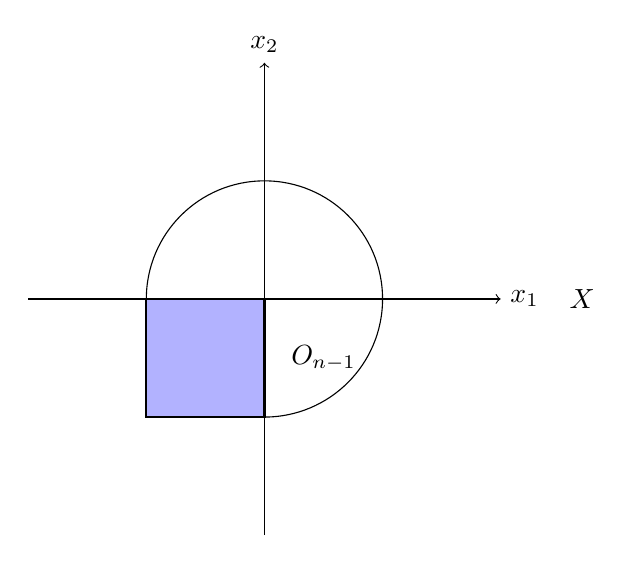
\begin{tikzpicture}[scale=1.5]
    % Draw the axes
    \draw[->] (-2,0) -- (2,0) node[right] {$x_1$};
    \draw[->] (0,-2) -- (0,2) node[above] {$x_2$};

    % Draw the circle
    \draw (0,0) circle (1);

    % Draw the shaded rectangle
    \filldraw[fill=blue!30, draw=black, thick, xshift=-1cm, yshift=-1cm] 
        (0,0) rectangle (1,1);
    
    % Label the point O_{n-1}
    \node at (0.5, -0.5) {$O_{n-1}$};
    
    % Draw the label X
    \draw (2.5, 0) node[right] {$X$};
\end{tikzpicture}

\end{document}